In order to derive the lower bound, we change our probabilistic model by introducing a set of latent variables $u$, so that
\begin{equation}\label{augmented_model}
	p(y, f, u) = p(y | f) p(f | u) p(u) = \prod_{i = 1}^n p(y_i | f_i) p(f|u) p(u).
\end{equation}

The corresponding graphical model is shown in fig. \ref{inducing_inputs_gm}. The values $u$ are considered to be the values of the same Gaussian process, from which the dataset is generated, at a set of points $Z = (z_1, \ldots, z_m)^T \in \R^{m \times d}$. Thus, the distribution $p(u)$ is given by 
$$p(u) = \N(u|0, K(Z, Z)).$$

Points $Z$ are called inducing points or inducing inputs. To make the formulas more clear, we will use a simpler notation for covariance matrices. We will denote $K(Z, Z)$ by $K_{mm}$, $K(X, Z)$ by $K_{nm}$, $K(Z, X)$ by $K_{mn}$, and $K(X, X)$ by $K_{nn}$.

We will refer to the introduced model as augmented model. Note that integrating (\ref{augmented_model}) with respect to $u$ we obtain the standard model (\ref{standard_model}).

\begin{figure}[!h]
	\centering
	\scalebox{0.9}{
		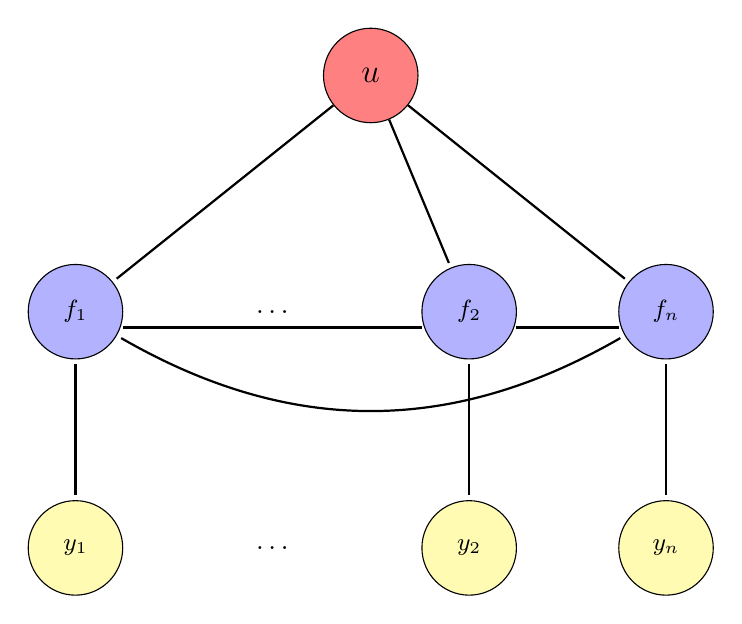
\begin{tikzpicture}
	\tikzstyle{x_i} = [circle, draw, fill=green!50, minimum size=1.2cm, text width=0.8cm, align=center, font=\large]
	\tikzstyle{f_i} = [circle, draw, fill=blue!30, minimum size=1.2cm, inner sep=2pt, outer sep=2pt, font=\small, align=center]
	\tikzstyle{y_i} = [circle, draw, fill=yellow!30, minimum size=1.2cm, inner sep=2pt, outer sep=2pt, font=\small, align=center]
	\tikzstyle{edge_label} = [font=\small, label={[label distance = -4pt]90:$\text$}]
	\tikzstyle{edge} = [thick, >=stealth]
	\tikzstyle{biedge} = [thick, >=stealth]
	\def\step{-3}
	\def\layerpos{3}

	\foreach \name/\x in {f_1/-2.5, f_2/2.5, f_n/5} 
	  	\node[f_i] (\name) at (\x, \layerpos) {$\name$};

	\draw[biedge] (f_1)++(0.6,-0.2) -- ++(3.8,0); %(f_2);
	\draw[biedge] (f_2)++(0.6,-0.2) -- +(1.3,0);% ++ (f_n);
	\draw [biedge] (f_1) to [out=-30,in=-150] (f_n);
	\node (other^2) at (0, \layerpos) {$\ldots$};

	%observables
	\pgfmathsetmacro{\layerpos}{\layerpos + \step}

	\foreach \name/\x in {y_1/-2.5, y_2/2.5, y_n/5} 
	  	\node[y_i] (\name) at (\x, \layerpos) {$\name$};

	\node (other^3) at (0, \layerpos) {$\ldots$};
	\foreach \from/\to in {f_1/y_1, f_2/y_2, f_n/y_n}
		\draw[edge] (\from) -- (\to);

	\tikzstyle{u} = [circle, draw, fill=red!50, minimum size=1.2cm, text width=0.8cm, align=center, font=\large]

	\pgfmathsetmacro{\layerpos}{\step/2}
	\node[u] (inputs) at (1.25, 6) {$u$};

	\foreach \to in {f_1, f_2, f_n}
		\draw[edge] (inputs) -- (\to);

\end{tikzpicture}
	}
	\caption{The augmented model}
	\label{inducing_inputs_gm}
\end{figure}

As $u$ and $f$ are generated from a Gaussian process with zero-mean prior, 
$$p(u) = \N(u|0, K_{mm}),$$
$$p(f|u) = \N (f|K_{nm} K_{mm}^{-1}u, \tilde K),$$
where $\tilde K = K_{nn} - K_{nm} K_{mm}^{-1} K_{mn}.$

Applying the standard variational lower bound (see, for example \cite{VarBayes}) to the augmented model, we obtain the following inequality.
$$\log p(y) \ge \E_{q(u, f)} \log \frac {p(y, u, f)}{q(u, f)} = \E_{q(u, f)}\log p(y | f) - \KL{q(u, f)} {p(u, f)},$$
for any distribution $q(u, f)$. This inequality becomes equality for the true posterior distribution $q(u, f) = p(u, f | y)$. We will restrict $q(u, f)$ to be of the form
$$q(u, f) = p(f | u) q(u),$$
where $q(u) = \N(u | \mu, \Sigma)$ for some $\mu \in \R^m$, $\Sigma \in \R^{m \times m}$.

This form of the variational distribution implies a Gaussian marginal distribution
$$q(f) = \int p(f | u) q(u) du = \N(f| K_{nm} K_{mm}^{-1} \mu, K_{nn} + K_{nm} K_{mm}^{-1}(\Sigma - K_{mm}) K_{mm}^{-1} K_{mn}).$$

As $\log p(y|f)$ depends on $u$ only through $f$, the expectation $\E_{q(u, f)}\log p(y | f) = \E_{q(f)}\log p(y | f)$. Now, as the likelihood factorizes over objects, $\E_{q(f)}\log p(y | f) = \sum_{i = 1}^{n} \E_{q(f_i)}\log p(y_i | f_i)$, where $q(f_i)$ is the marginal distribution of $q(f)$.

Finally, 
$$\KL{q(u, f)} {p(u, f)} = \KL{q(u) p(f | u)} {p(u) p(f | u)} = \KL{q(u)}{p(u)}.$$

Combining everything back together, we obtain the evidence lower bound
\begin{equation}
	\label{main_elbo}
	\log p(y) \ge \sum_{i = 1}^{n} \E_{q(f_i)} \log p(y_i | f_i) - \KL{q(u)} {p(u)}.
\end{equation}

Note that the KL-divergence term in the lower bound (\ref{main_elbo}) can be computed analytically, as it is a KL-divergence between two normal distributions. The expectations $\E_{q(f_i)} \log p(y_i | f_i)$ can be computed analytically in case of the regression problem. In case of classification we have to use integral approximating techniques in order to compute these one-dimensional integrals.

The evidence lower bound (ELBO) (\ref{main_elbo}) can be maximized with respect to variational parameters $\mu$, $\Sigma$ and kernel hyper-parameters. Using the optimal distribution $q(u)$, we can perform predictions for new data point $x_*$ as follows
$$p(f_* | y) = \int p(f_* | f, u) p(f| u, y) p(u | y) du df \approx \int p(f_* | f, u) p(f| u) q(u) du df = \int p(f_* | u) q(u) du.$$

This integral is tractable and
$$p(f_* | y) \approx \N(f| K(x_*, Z) K_{mm}^{-1} \mu, K(x_*, x_*) + K(x_*, Z) K_{mm}^{-1}(\Sigma - K_{mm}) K_{mm}^{-1} K(Z, x_*)).$$

Below we will consider three different methods for optimizing the lower bound (\ref{main_elbo}).

